In this chapter we present our work on estimating the uncertainty
in the predictions of online decision trees. We define the problem
and present some related work in Section \ref{sec:uncertain-trees-background},
describe the two algorithms developed for this purpose in Section
\ref{sec:uncertain-trees-method} and present our empirical evaluation
results in Section \ref{sec:uncertain-trees-results}.
We close the chapter with a discussion placing the work in the
context of our original research question in Section \ref{sec:uncertain-trees-discussion}.

\section{Background}
\label{sec:uncertain-trees-background}

As machine learning methods mature and become increasingly popular, they are more
often being deployed in critical scenarios were mistakes can be costly. Such
domains include autonomous vehicles, and the medical and financial sector.
In order for critical decision-making to be done by learning algorithms in these areas, we need
to have a notion uncertainty in the algorithms' predictions.
Some of these critical domains also include the requirement that critical decisions
be made in real-time in a constantly evolving environment, and under a tight computational budget. Examples include the financial domain \cite{streaming-finance} and autonomous vehicles \cite{av-safety}.

These examples demonstrate the need for highly accurate algorithms that can be trained
online, adapt to an evolving environment, and quantify the uncertainty in their
predictions. Most of the online learning methods available today do not offer
quantification in their predictions, while most methods that provide uncertainty
estimates are designed for the batch domain where the data are static and bounded.
In this work we aim to provide highly accurate algorithms that can be trained
online, on a sequentially arriving and potentially unbounded dataset, that also
provide uncertainty estimates for their predictions.

We develop two algorithms, one based on conformal prediction~\cite{vovk2005algorithmic} and one based on quantile
regression forests~\cite{meinshausen2006quantile}. The two algorithms are general random forest learners that
enable high accuracy \cite{hundreds-classifiers}, are computationally bounded
and adapt to concept drift through the use of online base learners \cite{fimt},
and provide uncertainty estimates at an accuracy level equal to or better
than the state of the art \cite{mondrian-forests-original}, while being an order of magnitude faster to run.

\section{Uncertainty Estimation for Ensembles of Online Decision Trees}
\label{sec:uncertain-trees-method}

In this section we provide an overview of the methods developed for this work.
We provide a brief description of the batch algorithms that we base our algorithms
on, and proceed to explain how we make use of approximations to transfer them to
the online domain. We deal with the regression, and our task is to develop algorithms
that exhibit what is called \emph{conservative validity} in conformal prediction literature. This refers
to algorithms that produce predictive intervals such that the probability of the true value not
being part of the interval is \emph{less than or equal to} $\alpha$, which is referred
to as the \emph{significance level}. This task is different from quantile regression \cite{koenker2005qr}
where the objective is for the error level to be \emph{exactly} $\alpha$.

\subsection{Inductive Conformal Prediction}

Conformal prediction (CP) is a meta-algorithm that can add the ability to
produce \emph{prediction regions}, that is, sets of classes for classification or
intervals for regression, to any point-prediction algorithm. It works by
quantifying how surprising or \emph{non-conforming} an instance is compared
to what the learner has observed and producing a region that is guaranteed
to contain the true value at a requested degree of certainty. CP is rigorously
proven to be \textit{valid}~\cite{vovk2005algorithmic}, that is, the probability of error is bounded
by the pre-selected \emph{significance level}.

While CP was originally proposed as an online learning framework, its computational
requirements made it impractical for large scale data, as it required to re-train
the model from scratch with the complete dataset for each incoming example.
\citet{papadopoulos2002icp} proposed \emph{Inductive Conformal Prediction} (ICP) as
a way to bound the computational cost of the method in the batch setting.
Instead of constantly re-training the learner, it sets aside a subset
of the training examples referred to as the \emph{calibration set},
and uses this to determine the non-conformity scores of the examples
and determine the intervals.

However, ICP is an offline method designed for the batch setting and assumes that the complete
dataset is available at training time, in addition to requiring a external
validation set to use as the calibration set. As such it cannot be applied to
the online domain.


\subsection{Quantile Regression Forests}

Quantile Regression Forests (QRF) \cite{meinshausen2006quantile} are an extension to
the random forest \cite{random-forests} algorithm that enables estimation
of the full conditional cumulative distribution function (CDF) instead of only
the conditional mean. Using the conditional CDF we can estimate prediction
intervals for a given significance level by computing the quantiles at the
edges of that interval. For example, for a significance level of 0.1,
we can take the 0.05 and 0.95 conditional CDF values to produce the interval.

QRF works by maintaining at the leafs not just the mean label value of all
the data points that get routed to that leaf, but maintaining a mapping
from every instance to its label in its leafs. Otherwise, it grows trees
like a regular random forest model. QRF uses a weighted sum of all the label
values to determine the CDF estimates.

However because QRF requires access to the complete dataset and needs to maintain
a mapping from each instance to its label value, it can cannot be used in an online
setting where instances arrive in sequence, and memory is bounded.

\subsection{Conformal Prediction with Online Regression Forests}

Our algorithm adapts ICP to the online setting by using online tree learners
to always maintain an up-to-date model, and uses a bounded FIFO queue of instances
as its calibration set to keep the memory requirements of the algorithm bounded. We make use of
out-of-bag examples from the bagging process in order to remove the need
for a separate calibration set, as done in \cite{rf-cp-oob}. We make use of
the online bagging algorithm by \citet{Oza2001online} and the online
regression trees by \citet{fimt} to develop online regression forests
that produce confidence intervals.

The algorithm works by maintaining a bounded FIFO queue of examples
that are used as the calibration set for the CP algorithm. This set
gets populated whenever an example is out-of-bag for at least one
tree in the ensemble. In the online bagging algorithm we are using,
a draw from a Poisson distribution is made for a each incoming instance,
for each learner in the ensemble. If the drawn sample is not larger
than zero, that example is out-of-bag for the learner and we add it
to the calibration set. We maintain a sorted list of predictions for the
examples that are out-of-bag which give us the \emph{non-conformity}
scores for the set.

At prediction time, we use these non-conformity scores to produce the
intervals: After a regular ensemble prediction is made for the incoming
instance, we determine the interval boundaries by moving through the
sorted list of non-conformity scores, and pick the value
$\phi = \calSet[\floor*{(1 - \significance) \cdot |\calSet|}$ to be half the
length of the interval, where $\calSet$ the sorted set of non-conformity scores
and \significance the requested significance level.
We call this meta-algorithm CPExact.

\subsubsection*{Approximations}

The map of predictors to out-of-bag predictions needs to be up-to-date with
the latest version of the predictors. That is, whenever an online learner
is modified, we need to update all its predictions in the calibration set.
In the worst case, it is possible that we will need to make $|\calSet| \cdot |L|$
predictions for a single incoming instance, where $L$ is the set of learners.
For a calibration set with thousands of instances and hundreds of trees in the ensemble, this can quickly
become computationally intractable. For this purpose we propose an approximate
version of the algorithm that only updates the predictions of the new
data points that have entered the calibration set since the last prediction.
This allows for significant computation savings, while still providing
an up to date representation of the data points' non-conformity, by constantly
adding new instances to the set and removing older ones. We call this
meta-algorithm CPApproximate.

\subsection{Online Quantile Regression Forests}

The batch QRF algorithm cannot be applied to the online setting as it requires
a mapping from the the complete set of instances to their labels to be stored
in memory at the leafs. The main idea for our algorithm is to use an approximate data
structure to store a sketch of the labels cumulative distribution at each leaf,
making it possible to estimate the quantiles from them.

To that end we use the state-of-the-art KLL quantile sketch \cite{karnin2016kll},
that gives a memory and computation-efficient way to approximate the CDF from
a stream of data. An important characteristic of the KLL sketch is that it is
\emph{mergeable}, that is, we can apply the sketch to different partitions of
a stream, and subsequently merge them, and the result should be the same
as if we had applied the sketch to the complete stream. We use this property
to make the predictions in our ensemble which are trained with samples of the
data.

We maintain  one of these sketches at every leaf in the trees of the ensemble.
For every incoming instance that gets filtered to a leaf, we update its sketch
with the label, thereby maintaining an up-to-date sketch of the CDF for every
leaf. At prediction time, we drop the instance
down every tree in the ensemble, and retrieve every sketch.
We can then merge those sketches together to extract the overall estimate
of the CDF for the ensemble.

\section{Main Findings}
\label{sec:uncertain-trees-results}

We evaluate our algorithms against a simple baseline and a state of the art
algorithm, Mondrian Forests (MF) \cite{mondrian-forests-original}. We use 20 small-scale
datasets gathered from the OpenML repository \cite{vanschoren2013openml}, as well
as 10 large scale datasets that exhibit concept drift. We note that while the approaches we developed are model-parallel, i.e.
every tree can be trained independently in parallel, the results listed are single-threaded
to ensure fair comparison with MF.

Evaluating interval prediction algorithms entails two aspects: The error rate
and the width of the intervals. The algorithms should maintain an error rate
that is below the significance level set by the user. However, this can be
easily achieved by producing very wide intervals that are uninformative.
For this reason we also need to take into account the width of  the intervals when
evaluating the quality of the predictions. We measure the actual error rate using Mean Error Rate (MER)
which is the mean of the 0-1 loss of the algorithm, and for interval size we compute
the Relative Interval Size (RIS) that
is the normalized mean size of the intervals produced.

To ease presentation we use two different metrics that
combine both aspects: the quantile loss \cite{koenker2005qr} and Utility,
based on the time-utility functions used in real-time systems \cite{tuf2005}.
Unlike quantile loss, Utility will only penalize methods that go above
the requested error rate, and as such is a better fit for our task.

We can see the results in terms of Utility for the small-scale data in Figure \ref{fig:utility-small-mid}
and for the large-scale drifting datasets in Figure \ref{fig:utility-concept-drift}.
We can see that our methods are able to outperform the Mondrian Forest baseline
in terms of Utility,
while at the same time being computationally more efficient. The runtimes for each
category of dataset are listed in Table \ref{tab:uncertain-runtimes}, where we
can see that our algorithms are up to an order magnitude faster
than Mondrian Forest.

\begin{table}
	\centering
	\begin{tabular}{l r r r r}
		\toprule
		Dataset      & MF  & OnlineQRF & CPApprox & CPExact  \\
		\midrule
		Small-scale data & 41.6       & 5.4     & 5.7      & 102.3        \\
		Flight delays   & 6340        & 836       & 899       & 27863        \\
		Friedman     & 2380      & 114      & 213      & 2011            \\
		\bottomrule
	\end{tabular}
	\caption{Average running times for all algorithms (seconds).}
	\label{tab:uncertain-runtimes}
\end{table}



\begin{figure}
	\centering
	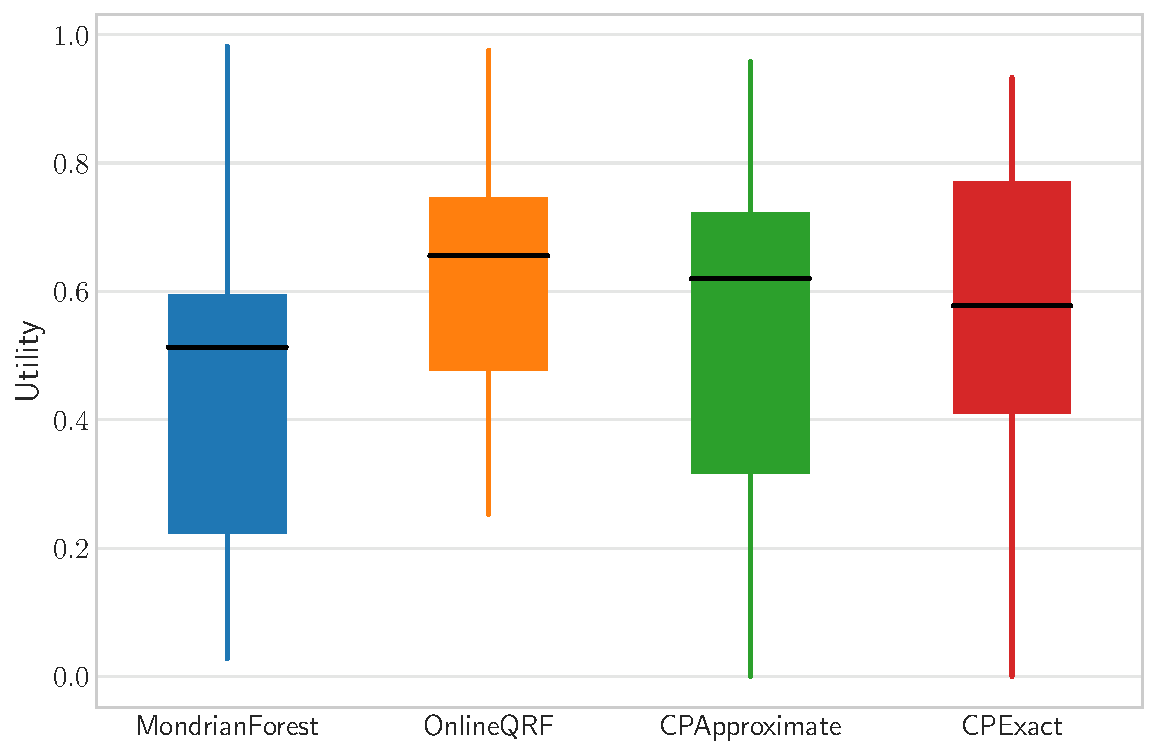
\includegraphics[width=0.8\columnwidth]{utility-small-mid}
	\caption{Utility for the small-scale data. Higher is better.}
	\label{fig:utility-small-mid}
\end{figure}

\begin{figure}
	\centering
	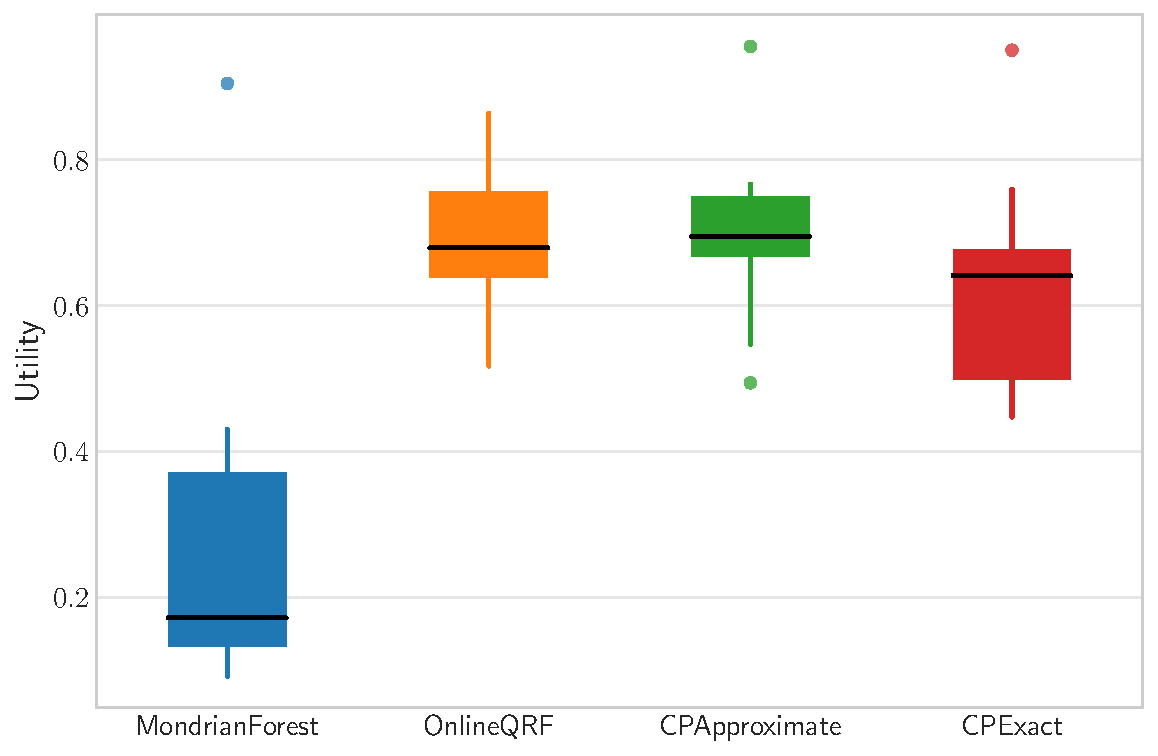
\includegraphics[width=0.8\columnwidth]{utility-concept_drift}
	\caption{Utility for the concept drift data. Higher is better.}
	\label{fig:utility-concept-drift}
\end{figure}

We also provide an evaluation for different significance levels.
Depending on the cost of making a mistake, we might require different levels of confidence
in our predictions. Thereby it's important to measure the performance of the
algorithms over a range of different significance levels. The results are listed
in Table \ref{tab:uncertain-significance} where we can see that Mondrian Forests cannot maintain the
error guarantees above 80\% confidence, and that OnlineQRF provides the best
compromise between maintaining the error rate below the requested level, while
keeping the produced intervals informative.

\begin{table}
	\centering
	\begin{tabular}{ll r r r r r}
		\toprule
		\multirow{2}{*}{Method} &  \multirow{2}{*}{Metric} &  \multicolumn{5}{c}{$\alpha$} \\
		\cmidrule(lr){3-7}
		& & 0.3 &   0.2 &   0.1 &   0.05 &   0.01 \\
		\midrule
		\multirow{2}{*}{MondrianForest}   & MER  & 0.28 & 0.20 & 0.13 &  0.094 &  0.062 \\
		& RIS  &  0.19 &  0.23 &  0.29 &   0.349 &   0.460 \\
		\midrule
		\multirow{2}{*}{OnlineQRF} & MER & 0.23 & 0.14 & 0.07 &  0.036 &  0.015 \\
		& RIS &  0.20 &  0.23 &  0.31 &   0.345 &   0.510 \\
		\midrule
		\multirow{2}{*}{CPApprox} & MER  & 0.22 & 0.13 & 0.06 &  0.032 &  0.006 \\
		& RIS &   0.21 &   0.31 &   0.48 &   0.785 &    1.130 \\
		\midrule
		\multirow{2}{*}{CPExact} & MER  & 0.25 & 0.16 & 0.08 &  0.039 &  0.009 \\
		& RIS &   0.28 &   0.37 &   0.57 &   0.622 &   0.944 \\
		\bottomrule
	\end{tabular}
	\caption{MER and RIS for different significance levels. The MER should be at most
		$\significance$ where $\significance$ the significance level.}
	\label{tab:uncertain-significance}
\end{table}

\section{Discussion}
\label{sec:uncertain-trees-discussion}

In this chapter we have presented our work on uncertainty estimation for
online decision trees. We developed two algorithms for this purpose,
and demonstrated their accuracy and efficiency compared to a state
of the art algorithm.

Connecting this work to our original goals in Section \ref{sec:intro-question-objectives},
we have dramatically reduced the computation necessary for online conformal
prediction by maintaining up-to-date online models. For both OnlineCP and
OnlineQRF we have bounded the memory use of the algorithms by using approximate
and bounded data structures, that are able to provide the estimates we need
at a fraction of the memory cost, compared to exact data structures.
The approximations made however create a tradeoff,
as we can no longer guarantee the consistency and validity of the algorithms.
In terms of communication cost, as the trees in a random forest are trained independently there is no
need to communicate model updates when running the algorithms in parallel.
However, for OnlineQRF in a distributed setting we would need to merge the histograms of each tree to provide
a quantile prediction. Through our use of the near-optimal KLL sketch we ensure
that the communication cost is minimal.
The optimizations listed cover two of the three objectives
listed in Section \ref{sec:intro-question-objectives} and this work investigates
an aspect of our research question in the context of uncertainty estimation.